%

%
%

%
%
%
%

%

%


\begin{figure}
%
{\small
\begin{minipage}{0.47\columnwidth}
\centering 
Input image \medskip

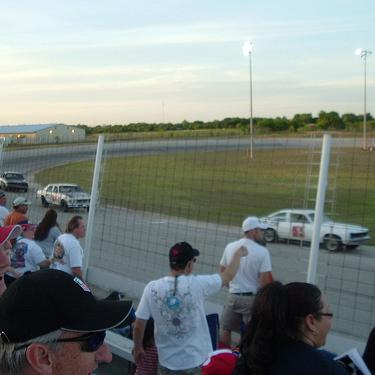
\includegraphics[width=\columnwidth]{figs/per_channel_maps/2/pos.jpg} 

\end{minipage}%
\hfill
%
\begin{minipage}{0.5\columnwidth}
\centering
resolution $s^*=224$ \\

$p^* = 1$ \hspace{1cm} $p^* = 3$ \\

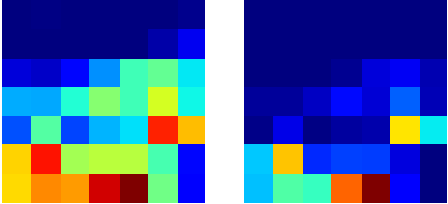
\includegraphics[width=0.8\columnwidth]{figs/per_channel_maps/2/activ_224.pdf}

full resolution \\

$p^* = 1$ \hspace{1cm} $p^* = 3$ \\

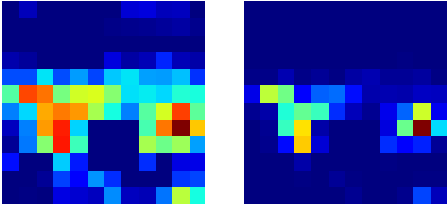
\includegraphics[width=0.8\columnwidth]{figs/per_channel_maps/2/activ_fullres.pdf}
\end{minipage}}
\vspace{-5pt}

\caption{\label{fig:heatmap}
    An off-the-shelf ResNet-50 reacts strongly on channel 909 of the last activation map for class ``racing car''. 
    The image on the left is a hard example for the class.     
    We show channel 909 for that image, at several resolutions and with GeM parameters $p^*=1$ and $p^*=3$.
   	In the low resolution version, the cars are too small to be visible individually on the activation map. 
	In the full resolution version, the location of the cars is more clear. 
	In addition, $p^*$\,$=$\,$3$ reduces the noisy detections relative to the true locations. 
}
\vspace{-7pt}
\end{figure}

%
%

%

%
%
%
%
%
%
%
%
